\chapter{Introduction}

\section {Motivation}

Single core performance in CPUs has stalled for the last 10 years as processor manufacturers focus on multi-core systems in order to increase performance \cite{procspeed}. Unfortunately software designed previously and some of the applications written recently do not take advantage of the parallelism in modern CPUs. This could have been considered unimportant or too difficult. Improving the performance of systems using such implementations is impossible, as upgrading hardware will not help anymore, but may sometimes be required after the system was developed.

Parallelizing existing software is a daunting proposition as it was not initially considered. The programmers involved need to identify the parts of the application that consume the most processing time and decide whether it is actually possible to improve them. This paper presents some tools to aid in such attempts.

In order to illustrate the usefulness of tools in the analysis of existing software we will present a simple example program in Figure \ref{cap1:emsim:seq}, which needs to be parallelized.

\begin{figure}
	\begin{center}
		\inputminted[linenos, fontsize=\scriptsize]{c}{emsim_seq.c}
	\end{center}
	\caption{EM Simulator sequential implementation}
	\label{cap1:emsim:seq}
\end{figure}

The user has determined that the loops present in this file take up almost all the execution time as can be seen in Figure \ref{cap1:emsim:profile} and he must determine if their iterations can be run in parallel. Intuitively no such knowledge can be gained as a thorough understanding of the application and careful analysis of the loops is required. The pointer arithmetic present in the loop 12 makes source code inspection very challenging and without understanding the logic behind the implementation it becomes impossible.

\begin{figure}[!ht]
	\centering
	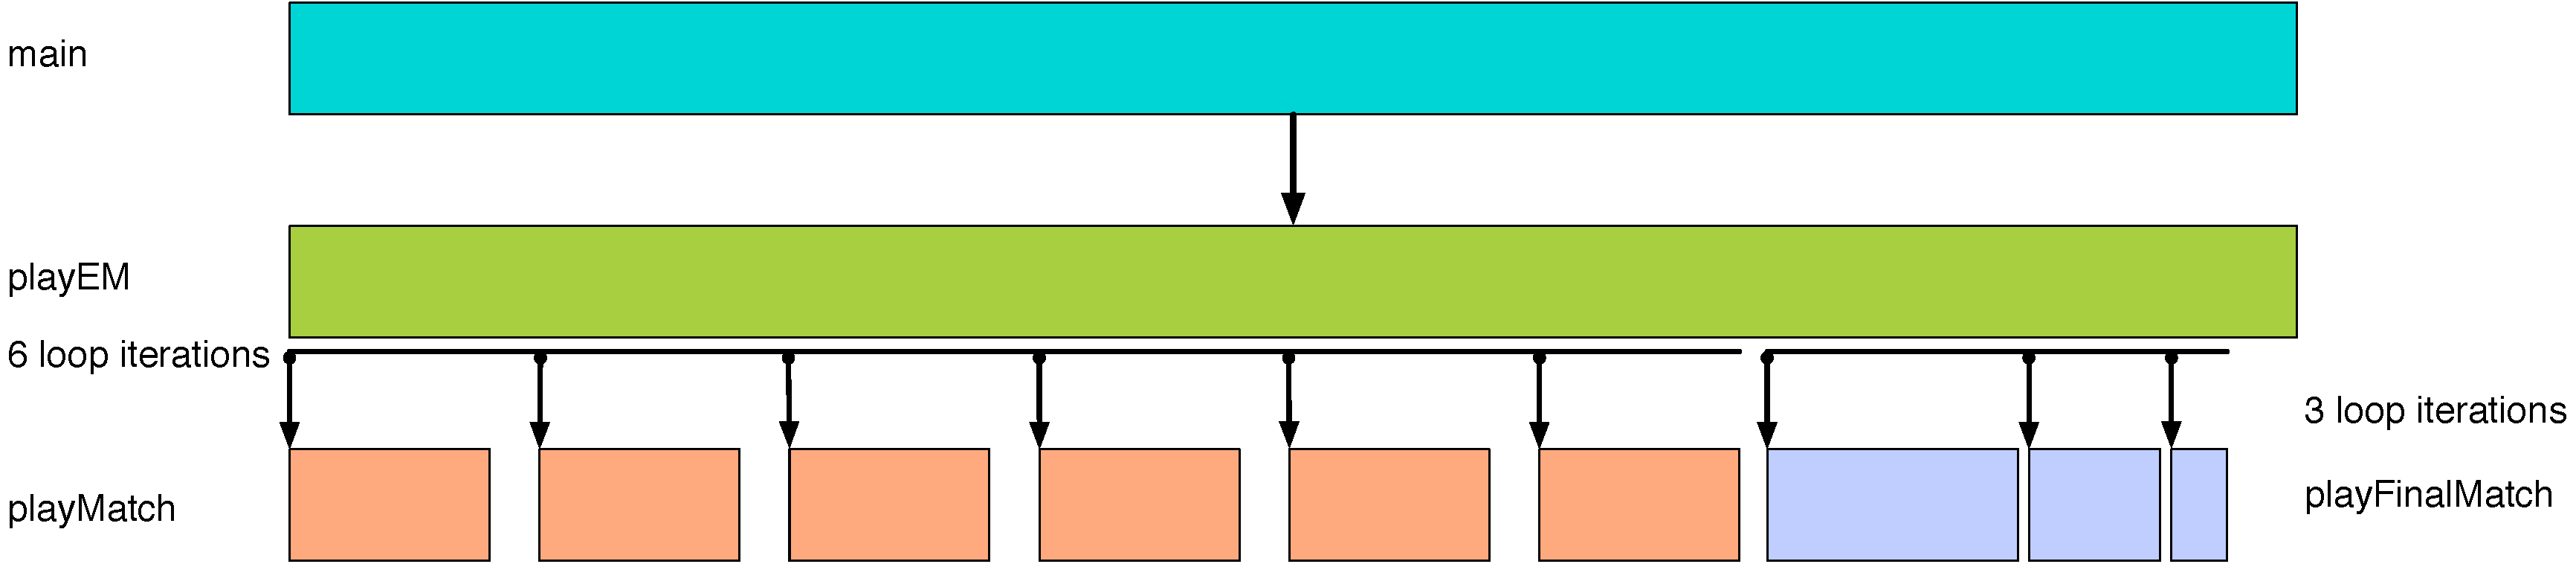
\includegraphics[width=0.8\textwidth]{emsimprofile}
	\caption{Profile view of the execution the code using Parceive}
	\label{cap1:emsim:profile}
\end{figure}

In contrast we show the visualizations of loops on lines 12 and 30 in Figures \ref{cap1:emsim:sections1} and \ref{cap1:emsim:sections2} respectively. There we can see the possible speedup when running on a machine with 4 threads and more importantly the actual conflicts that the user must resolve in order to maintain correctness. The loop on line 12 can be easily modified, even though all iterations work on the same arrays, since each iteration works on distinct elements.

\begin{figure}[!ht]
	\centering
	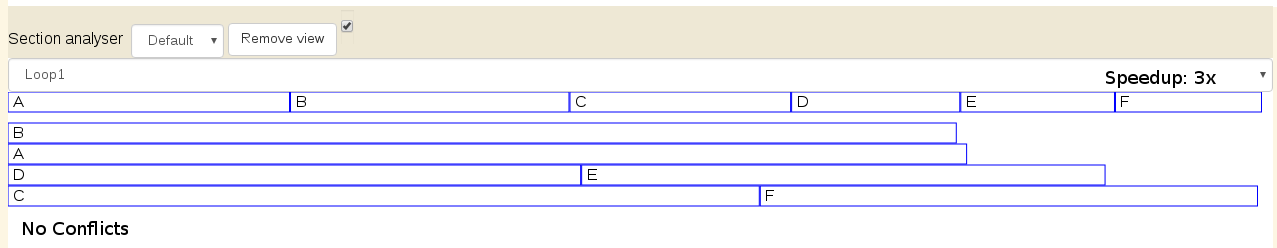
\includegraphics[width=0.8\textwidth]{loop1section}
	\caption{Section view of the loop on line 12 in Figure \ref{cap1:emsim:seq}}
	\label{cap1:emsim:sections1}
\end{figure}

\begin{figure}[!ht]
	\centering
	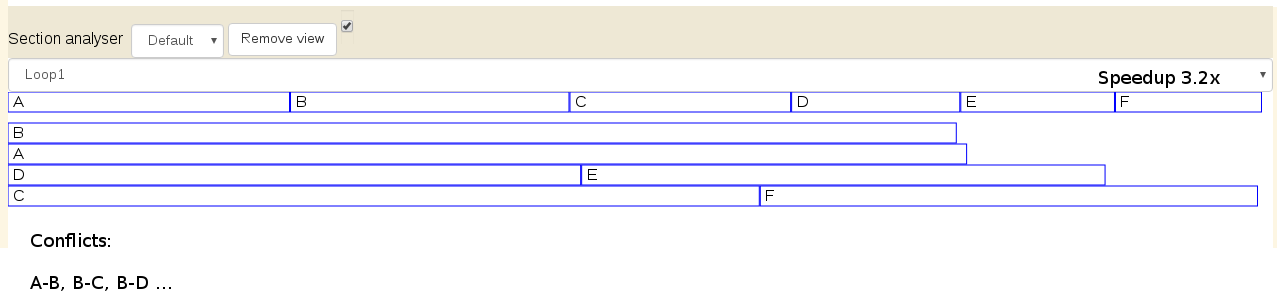
\includegraphics[width=0.8\textwidth]{loop2section}
	\caption{Section view of the loop on line 30 in Figure \ref{cap1:emsim:seq}}
	\label{cap1:emsim:sections2}
\end{figure}

As can be seen in these example, information about the program can be gained by automated tools. Profiling is a well known method of finding performance hot-spots in applications. In this paper we propose tools that can help determine the potential for parallelization of these bottlenecks.

\section {Contribution}

This paper presents two tools developed using Intel Pin that use dynamic instrumentation to obtain information about a sequential application. In order to utilize this data multiple visualizations were developed that help the user in determining which parts of an application can be parallelized.

The tools are based on the concept of tagging sections of a programs source code. In Figures \ref{cap1:emsim:sections1} and \ref{cap1:emsim:sections2} the loops are tagged as sections and each iteration starts a new task. The visualization presents the possible performance benefit and conflicts when running the tasks within a section in parallel.

An additional feature is available in this framework, pipeline analysis. Pipeline parallelism can be sometimes be applied to loops, despite the fact that iterations can not be run in parallel to each other. This approach splits each iteration into stages and different stages from different iterations can be run parallel to each other. As a simple example we consider file processing, where data is read, processed and written to another file. Individual iterations can not be run in parallel, but the io operations and the processing can be seen in Figure \ref{cap1:pipeline}. In Chapter §2 we will present a more concrete example, bzip compression.

\begin{figure}[!ht]
	\centering
	\begin{tabular}{ l | l | l | l | l}
		R & P & W & & \\
		\hline
		R &  & P & W & \\
		\hline
		R &  & & P & W \\
	\end{tabular}
	\caption{Pipeline, R - read, P - proecess, W - write}
	\label{cap1:pipeline}
\end{figure}

Tagging of the source code is done interactively and is applied dynamically to the program being instrumented. Changes to the source code of the applications are not required for this tool to function. This makes instrumenting a painless process on complex systems or when dealing with convoluted build processes.

\section {Related Work}

\subsection{Profiling}

The tools presented in this paper are able to gather profiling information about the application, but it is imprecise and slow in this regard. As such it is recommended to use an existing profiler to discover the performance bottlenecks. Our visualizations become useful only after this step.

\subsection{Parceive}

The implementation of this tool generates a database compatible with Parceive, keeping all of its existing views functional. The biggest difference is that additional information about tags is recorded, making our analysis possible. The tracing can also be controlled using tags, making it possible for large applications to be analyzed.

We have also created multiple new views that are designed to help a developer in analyzing parallelization opportunities. These visualizations are based on the framework provided by the Parceive UI.

\subsection{Intel Advisor}

The section analysis that this application provides is also possible in Intel Advisor, but with a different workflow. The source code of the application needs to be annotated using macros provided by the tool such as \texttt{ANNOTATE\_SITE\_BEGIN} or \texttt{ANNOTATE\_TASK\_BEGIN}. This requires rebuilding the application and then instrumenting it using Intel Pin. Our tool is able to instrument the application without the need for source code changes, reducing the number of steps required to gain information about the application.

Intel Advisor also offers many features not available in our tool such as vectorization and memory access pattern analysis. We expect the two tools to complement each other when trying to achieve the greatest performance gains.

\section {Outline}